\section{Implementering}\label{sec:deadline-implementation}

\subsubsection{Now og Wait}
Som vi beskrev i \des introducerede vi de to globale funktioner Now og Wait der hhv. returnerer tiden og før en proces til at vente i et givent tidsrum. Vi har ændret den interne implementering af funktionerne, så de bruger realtid. Dette sikre en ensartet implementering af tid på tværs af de tre udviklede versioner af TimedPyCSP. Det vil være en fordel hvis greenlet versionen også brugte Now, når den skal bruge tid, i hvilket tilfælde, det kunne fjernes helt i denne version. 

\subsubsection{Overskreden deadlines}
Planlægning i realtime kræver man tager stilling til  hvordan  overskredne deadlines skal håndteres. Man kan vælge enten at se det som en egenskab for processen hvor dens deadline enten kan være overholdt eller ej. Alternativt kan der kan en overskreden deadline resultere i en exception.

Hvilken metode der egner sig bedst til RTP afhænger af hvilken deadline der er tilknyttet processen. Er der tilknyttet en soft deadline til en proces, vil processen stadig tilføje værdi til systemet, selvom det  overskrider dens deadline. Hvorfor  det stadig er bedst for systemet at udføre processen færdig. I dette tilfælde  skal systemet blot markere at dens deadline er overskredet, og senere må programmøren så manuelt håndtere at processens deadline er overskredet. 


Hvis en proces har tilknyttet  en hard deadline, vil en overskredet deadline  ikke tilføje værdi til systemet og derfor kan det ikke betale sig for systemet at lade processen blive færdig. processen skal derimod stoppes hurtigst muligt, så systemet i stedet kan udføre processer hvis deadline endnu ikke er overskredet. For et system hvor processerne har hard deadlines vil det derfor være bedst hvis en overskredet deadline resulter i en exception, der med det samme stopper processen og lader programmøren bestemme hvordan processen skal forholde sig til at deadlinen er overskredet.

Vi har valgt at der i vores system skal kaldes en exception hvis en deadline overskrides. Dette er er gjort ud fra en betragtning om at systemet ikke kender konsekvensen af en overskredet deadline, men på processniveau har programmøren tilføjet en deadline og derfor må det være programmørens ansvar at håndtere processen ved en overskridelse af deadline.  Hvis processen stadig kan bidrage med værdi, kan programmøren lade processen fortsætte sin kørsel, og alternativ kan processen lukkes korrekt ned. Ulempen ved at kalde en exception er at processen stopper sin eksekvering i utide, som kan give problemer f.eks. hvis processen er tilknyttet en kanal og venter på at kommunikere.  Kanalerne holder i \pycsp styr på antallet af processer der vil kommunikere og hvis processen pludseligt forsvinder vil tilstandsvariablerne ikke være sat korrekt. det er derfor vigtigt at processen manuelt rydder op efter sig selv i forbindelse med en exception, da det ellers kan resultere i et ustabilt system.

I en fremtidig version, vil man kunne udvide muligheden med et hybridversion der både kan håndtere processer med soft deadlines, der skal markeres samt og kan kalde en exception ved processer med hard deadline. Processen kan f.eks have  tilknyttet dens type af deadline. Systemet kan så reagere passende efter typen af deadlines, så soft deadlines blev færdigbehandlet, mens hard deadlines resulter i en exception.


\subsubsection{Ændringer i \sched en}
I \code{greenlets} versionen af \sched en findes der som nævnt i \cref{sec:scheduler} tre lister af processer: \code{new}, \code{next} og \code{timers}. De tre lister er prioriteret således at der først kigges på processer fra \code{timers}, dernæst fra \code{new}, og til sidst kigges der i \code{Next}.

I RTP er det ikke hensigtsmæssigt at inddele processerne i disse tre  kategorier. Vi skal derimod have et miljø der gnidningsløst tillader både processer med og uden deadlines, samt at de dynamisk kan ændres. \sched en skal i forbindelses med processkift hurtigt kunne finde den den næste proces der skal udføres.

Vi har derfor valgt at fjerne  de tre lister og erstatte dem  med \code{has\_priority},  \code{no\_priority} og \code{timers}. \code{has\_priority} og  \code{no\_priority}  bruges til at placere  aktive processer der ønsker at blive udført, mens  \code{timers} er en kopi af \des versionen. 

Vigtigt at gøre sig bemærket med processer der ligger i timers, er at de enten har kaldt en timeout i forbindelse med en \code{alternation}, eller har kaldt funktionen  \code{Wait}. Her kan forventer en programmør at processen vil vente i præcist det angivede tidsrum, men dette er kun  muligt i \des versionen hvor tiden står stille. I versionen hvor tiden er reel fortolkes de to funktioner som at processen skal vente  minimum det angivne tidsrum. I \code{greenlets} versionen  aktivere man  først processer fra timers listen for at minimere overskridelsen fra processen afgiver kontrol til den igen har kontrol til den igen er aktiveret. På denne måde emuleres at processen venter præcist i tidsrummet man har angivet for så at fortsætte. I RTP formodes at der findes en mængde processer der skal gennemføres inden en deadline hvorfor de må kæmpe om CPU-tid. En proces der har ventet i timers listen skal derfor ikke nødvendigvis udføres med det sammen, da det hele tiden bør være processen med højst prioritet der skal udføres, uafhængigt af processerne i timers hoben. Processerne der ikke længere skal ligge i timeout, bliver derfor kun planlagt på lige fod med de andre processer og må derefter kappes om at være den optimale proces der udvælges til kørsel.

Til at implementere \code{has\_priority} bruger vi også en hob, men da modulet heapq  kun understøtter min hobe kan vi ikke lave en klassisk prioritetshob, da den skal kunne udtrække processen med maksimal prioritet. Vi har dermed to muligheder, enten kan vi lave vores egen implementering af en maks hob eller ændre vores prioriteter internt så en lav værdi angiver en høj prioritet. Med en egen implementering har vi en  logisk opbygning af prioriteter, men vi får ikke fordelenen ved den underliggende implementering  direkte i C, som man opnår ved brug af modulet heapq. Vælger vi at bruge modulet heapq skal vi invertere prioritetsbegrebet, så det er den laveste prioritet der udvælges først. Dette viser  sig dog ikke at være et problem  i vores tilfælde da vi ønsker at benytte os af en EDF algoritme og derfor nemt kan opnå den ønskede effekt ved at bruge en proces deadline som dens prioritet. Her vil en lav deadline betyde at processen snart skal være færdig hvilket resulterer i en høj prioritet.
Vi kan derfor blot benytte en proces deadline som dens prioritet og benytte en min hob. Hvis man i en fremtidig version ønsker at processerne kan have en valgfri prioritet, kan man f.eks implementere dette ved efterfølgende at mindske prioriteten yderligere. Dette vil resultere i at processen bliver opprioriteret ifh. til andre processer.

\subsubsection{Preempting}

Som vi har beskrevet i \cref{sec:rtp-pycsp}, kan  man risikere at en proces med lav prioritet proces og lang kørselstid kan blokere for en proces med høj prioritet. 
Her konkluderede vi at det er programmørens opgave at processen afgiver kontrol, og derfor skal det være nemt at afgive kontrollen fra processen. til dette har vi lavet funktionen \code{Release()}, der minder om \code{Yield} for \code{co-rutiner}.

Implementeringen er meget simpel og er blot en wrapperfunktion, da den underliggende funktionalitet allerede eksisterer. Den aktive proces stopper og bliver genplanlagt til senere kørsel af \sched en. Dermed ligges processen på den relevante kø og  \sched en  kan blot vælge  den bedst proces der skal udføres. Er  der ikke kommet ny processer vil det stadigt være den originale proces der udføres og kan fortsætte sin kørsel. Hvis der derimod i mellemtiden er ankommet en eller flere nye processer der har højere prioritet, vil disse blive udført i stedet.

Problemet ved denne tvungne procesafgivelse er at det kan tage lang tid at blive lagt korrekt i en min\_hob, som vil være spildt hvis den alligevel med det samme fjernes fra køen. Man vil derfor nok i en senere version kunne optimere hastigheden af \code{Release()}.


\subsubsection{Udvidelse af \code{Process}}

Hver proces skal have mulighed for at få tilknyttet en deadline, og desuden skal det være muligt i forbindelse med prioritetsnedarvning midlertidigt at kunne ændre dens prioritet til en kunstig prioritet.

Når en proces bliver udsat for prioritetsnedarvning, skal systemet planlægge processen ifh. til den nye kunstige prioritet. Men det er ikke defineret om den kunstige prioritet medfører at systemet kaster en  \code{deadlineException},  hvis  denne overskrides. Ved at kaste en \code{deadlineException} i processer med kunstig prioritet, kan programmøren se præcist hvilken proces der arbejder, og dermed bedre debugge hvorfor den originale proces også kaster en \code{deadlineException}. \Cref{fig:producer-worker-consumer} viser at med en \code{deadlineException} vil det tydeligt fremgå at det er $B2$ der bære skylden for at deadlinen ikke overholdes.

En anden begrundelse for at lade en kunstig prioritet medføre en \code{deadlineException}, er hvis processerne findes i et generator/arbejder/forbruger-netværk, som vist i \cref{fig:producer-worker-consumer}. Her tilføjes forbrugeren og generatoren for den kunstige prioritet. Hvis denne deadline ikke nås er dataen som arbejderen bearbejde ikke længere relevant og arbejderen bør derfor stoppe det irrelevante arbejde snarest. Dette ville medfører at $B_2$ kunne stoppe sit arbejde i til $t = 5$ i modsætning til at fortsætte til $t = 6$.



\begin{figure}
 \begin{center}
  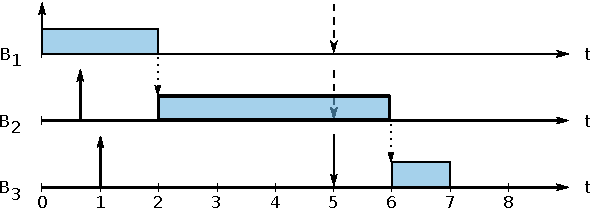
\includegraphics[scale=1.00]{images/producer-worker-consumer}
  \caption{Et generator/arbejder/forbruger -netværk. De stiplede pile i proces $B_1$ og $B_2$ til $t=5$ viser en kunstig prioritet på baggrund af $B_3$'s deadline. Den lille stiplede pil mellem  $B_1$ og $B_2$ i $t=2$ og mellem $B_2$ og $B_3$ i $t=6$ viser kommunikation mellem processerne.}
  \label{fig:producer-worker-consumer}
  \end{center}
\end{figure}

\begin{figure}
 \begin{center}
  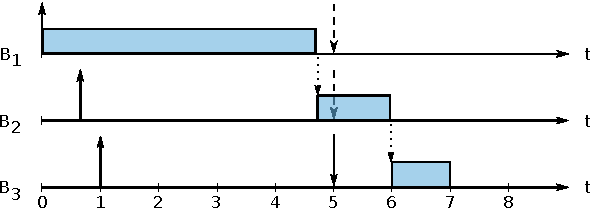
\includegraphics[scale=1.00]{images/producer-worker-consumer2}
  \caption{Samme netværk som i \autoref{fig:producer-worker-consumer}, men i dette tilfælde venter $B_2$  på data fra $B_1$ i hovedparten af tiden inden en deadline.}
  \label{fig:producer-worker-consumer2}
  \end{center}
\end{figure}


Der er dog flere problemer ved at lade en kunstig prioritet medføre en \code{deadlineException}.  Til at hjælpe programmøren,  er det ikke givet at den proces der overskrider en deadline, er den der har brugt tiden. \CRef{fig:producer-worker-consumer2} viser næsten netværk som før,men i dette tilfælde bliver data først sendt fra $B_1$ umiddelbart før en overskridelse af deadline. Her vil det fremgå for programmøren  at det er $B_2$ der er ansvarlig for overskridelsen og ikke $B_1$. Dermed mister \code{deadlineException} sin troværdighed til debugging. I CSP findes desuden begrebet traces, som kan bruges til at se hele forløbet for et program. På nuværende tidspunkt arbejdes der med at introducere traces til \pycsp og når dette er færdigt, vil det være et langt at foretrække som værktøj til debugging.

Et andet problem ved at kaste en \code{deadlineException} ved kunstigt lave prioriteter, er at processer måske  ikke er designet med hensyn til en mulig \code{deadlineException}. Programmøren skal dermed sikrer alle sine processer, hvis ikke hele processen skal risikere at stoppe ved en exception der ikke bliver hånteret korrekt. Begrundelsen for en deadline, og den tilhørende \code{deadlineException}, er kontekstafhængig, og  det er ikke sikkert processen kender begrundelsen for en given deadline, og vil  ikke kunne reagere optimalt. Eksempelvis  vil $B_2$ fra eksemplerne, ikke uden  forhåndsvidden kunne foretage valget om en \code{deadlineException} betyder den skal sende sit arbejde uafhængigt af hvor langt den er kommet. Stoppe arbejdet til den bliver bedt om at fortsætte. eller smide arbejdet ud og starte bearbejdningen af nyt data.

Vi har derfor valgt at det kun er processer med en eksplicit deadline, der har mulighed for at kaste en \code{deadlineException}. Processer der nedaver en prioritet bliver planlagt i henhold til den højeste prioritet de har, og vil altid  gøre arbejdet færdigt. En proces skal dermed kunne adskille sin egen deadline fra den prioritet som den skal planlægges med, til trods for de to tal i en stor del af tiden vil være det samme.

Vi har valgt at udvide procesmodellen med variablen \code{deadline}, der indeholder den specifikke deadline for processen, og som dikterer om der skal kastes en 
\code{deadlineException}. Desuden tilføjer vi listen \code{inherit\_priotity}, som indeholder de aktuelle prioriteter for processen. Når andre processer ønsker midlertidigt at ændre en proces prioritet, tilføjes den listen. Ved at bruge en liste i stedet for blot en variable, har processen mulighed for at blive opprioriteret flere gange, og vende tilbage den oprindelige prioritet efterfølgende. Når en proces får en eksplicit deadline, tilføjes denne værdi også til listen, som dens startprioritet. 

Når \sched en placere processen i sin bob bruges blot den mindste prioritet i listen ihh. til vores implementering af \sched en. Dette medfører  at når en proces efterfølgende  får ændret i sin liste af prioriteter skal processen genplanlægges for at sikre den står på den korrekte plads i min-hoben i \sched en. 

\subsubsection*{Kanaler}
I \pycsp findes der kun kanaler af type \code{Any-To-Any} og derfor kan der altid  være et vilkårligt antal kanalender i hver enden af kanalen, der måske er klar til at kommunikere. Vi skal derfor ændre koden, således at kommunikationen mellem kanalenderne altid foregår mellem de højst prioriterede processer. 

I greenletsversionen foregår udvælgelsen af kanalender til kommunikation ved hjælp af funktionen \code{match}, der udnytter at  hver kanal vedligeholder to lister af processer for hhv. de processer der ønsker at sende og modtage data på kanalen. Når en proces eks. ønsker at modtage data tilføjer den sig selv til listen af processer der ønsker at modtage, og prøver derefter i \code{match} funktionen at finde en proces der vil sende data. Er der ingen processer der venter på at sende data, venter processen selv  på at en proces melder sig klar til at sende data, og som så vil kalde \code{match}. Til hver vellykket kommunikation af data vil \code{match} altid blive kaldt to gange, hvor kun den sidste vil resultere i at kommunikationen lykkedes.

Ideen bag funktionen \code{match} er enkel og  udnytter at greenletsversionen er enkelttrådet så hver proces kan løbe listerne igennem uden andre processer ændre på listernes tilstand.  Vi er kommet frem til at  en simpel sortering af listerne, med hensyn til deres interne prioritet vil resultere i det altid er den højst prioriterede proces der indgår i kommunikationen. Den ændrede match kan ses i \cref{lst:match}, hvor det kun er linje 119 og 120 der er ændret.

\begin{lstlisting}[firstnumber=117 ,float=hbtp, label=lst:match, caption=funktionen \code{match} der sorterer kanalrequests.]
def match(self):        
    if self.readqueue and self.writequeue:
        self.readqueue.sort(key=lambda channelReq:channelReq.process.internal_priority)
        self.writequeue.sort(key=lambda channelReq:channelReq.process.internal_priority)
        for w in self.writequeue:
            for r in self.readqueue:
                if w.offer(r):
                    return       
\end{lstlisting}

Funktionen \code{match} vil blive kaldt en gang for hver proces der ønsker at kommunikere, og derfor vil listerne til hvert kald af \code{match} være totalt sorteret minus det sidste element i listen. Desuden vil der altid i den ene liste maksimalt være et element der er aktiv, hvorfor den ene liste højst sandsynlig vil være kort kørselstiden for de to sorteringer vil derfor være lille. Bemærk desuden at listerne er sorteret så værdien af den interne prioritet er stigende, og derfor er det processen med lavest værdi, der først bliver udvalgt til et match, i overensstemmelse med repræsentationen af prioriteter som nævnt i afsnittet ``Ændringer i \sched en''.

\subsubsection*{Alternation}

Som  beskrevet af \citeauthor{Burns1990}, opstår der en konflikt ved brugen af  prioriterede valg. ifh. til prioriteter på processer \cite{Burns1990}. De beskriver en kodestump som angivet i \cref{lst:pri-select}, hvor processernes prioritet er angivet som Pri1 og Pri2, og hvilken proces der udvælges afhænger af processernes indbyrdes forhold som angivet i \cref{tab:prioritizedSelect}.


\begin{lstlisting}[firstnumber=1 ,float=hbtp, label=lst:pri-select, caption={ (priority) select. Eksemplet er kopieret fra \cite[160]{Burns1990}}]
(priority) select
   A1 -- Process P1
 or
   A2 -- Process P2
 end select
\end{lstlisting}

\begin{longtable}{lccc}
   	\toprule
    &Pri1 > Pri2 & Pri1 = Pri2 & Pri1 < Pri2\\
    \midrule
    \endfirsthead 
    \toprule
    &Pri1 > Pri2 & Pri1 = Pri2 & Pri1 < Pri2\\
    \midrule
    \endhead % slut efterfølgende headere
    \bottomrule
    \multicolumn{4}{r}{\textit{fortsættes}}
    \endfoot % slut footer
    \bottomrule
	\caption[]{Konflikten ved brug af prioriteret valg og procesprioriteter. Eksemplet er kopieret fra \cite[160]{Burns1990}}\\
	\label{tab:prioritizedSelect}
    \endlastfoot % slut sidste footer
      	select          & A1 & Arbitrary    & A2 \\
		priority select & A1 & A1           & ? \\    
\end{longtable}

I \pycsp findes der kun en prioritets valg, og dermed kan vi se bort fra første række af \cref{tab:prioritizedSelect}, og konstatere at vi introducerer  en konflikt med introduktionen af prioriteter. For \citeauthor{Burns1990} er løsningen en ``orthogonal solutions'', der  tager hånd om begge typer af prioriteter. De  vage  i deres løsning, men ønsker overordnet set to typer, Weak og Strong Select. Hvor Weak select sorteres primært ifh. til processernes prioritet og sekundært efter det prioriterede valg. Strong select udvælger modsat udelukkende processer efter det prioriterede valg. De forestiller sig at primært skal weak select bruges, men i hjørnetilfælde skal en programmør have mulighed for at tvinge en prioriteret valg igennem

Vi ønsker en løsning så en alternation i \pycsp  minder om weak select. Dvs at først skal der kigges der på om alternation kan vælge en guard umiddelbart. Hvis der er minimum en guard klar foretages der et prioriteret valg baseret på først processernes prioritet, og hvis flere processer har samme prioritet  foretages det prioriterede valg. Er ingen guards klar bør processen vente i dens alternation, og vælge den første guard der bliver klar, uden at skele til dens prioritet.

I artiklen fra \citeauthor{Burns1990}  udvælger man en proces blandt flere mulige, mens en \code{alternation} udvælger en kanal der i \pycsp er af typen any-to-any. Dette medfører at man ikke  foretager et valg mellem processer, men foretager et valg mellem kanaler, som processen kommunikerer med. For at foretage en weak selection i vores \code{alternation}, skal man derfor kunne finde prioriteten for kanalerne. Dette findes ikke, men vi kan emulere at en kanal har  prioritet, ved at finde den højst prioriterede proces i hver kanal der er interesseret i kommunikation.  Vi har derfor lavet to hjælpefunktioner der finder de højst prioriterede processer der er villig til hhv. at sende og modtage data. Med disse hjælpefunktioner kan vi til hver kanal se på om det er en input- eller output-guard, der knytter sig til kanalen og finde den tilhørende prioritet for kanalen. \inline{Skal det begrundes hvorfor vi har to hjælpefunktioner}
\fxnote{skal det afsluttes bedre?}




\begin{itemize}
\tightlist
\item Process udvidet med: \\self.inherit\_priotity = []     \\
            if isinstance(arg, pycsp.greenlets.channelend.ChannelEndRead):\\
                arg.channel.\_addReaderProcess(self)\\
            if isinstance(arg, pycsp.greenlets.channelend.ChannelEndWrite):\\
                arg.channel.\_addWriterProcess(self)
\item Channel:\\
        self.readerprocesses = []\\
        self.writerprocesses = []

\item Udviddet \_read og \_write
\item Udvidder match
\item     def choose(self) i alternation


\end{itemize}
